\section{Optimal number of hash functions}
\label{sec:optimalk}
Classically, the optimal number of hash function is derived through finding the extrema of the asymptotic formula for $f_{bloom}$ given in Eq. \ref{fBloom} as :
\begin{equation}
\label{eq:kopt}
k^*_{bloom}=\frac{m}{n}\ln 2
\end{equation}
However, as we said, the underlying formula for FP probability is not fully correct, so we need new means of deriving the optimal value of $k$, minimizing the FP probability for a given BF size $m$ and number of inserted elements $n$.
\subsection{Deriving the optimal $k$}
We derive the optimal value of $k$ through a side observation relating to the compression theorem in information entropy theory. One can see a Bloom Filter as a coding scheme enabling to represent the set $\mathcal{S}$ of $n$ entries that are inserted in it. In order to be the most efficient space-wise, one would be expected that the bit array of the BF is the most compact and compressed one. Now we can assume that the Bloom filter is an array of $m$ independent bits. If the array of $m$ bits is such that one can compress into another array of $m'$ bits without any loss, we can build a new BF with array length $m'$ that will have the same performance as the $m$ bits array. The compression theorem in Information theory \cite{shannon} ensures that an $m$ bits sequence cannot be more compressed if its entropy defined as:
\begin{equation}
h=-\left(p'\log_2 p' +(1-p')\log_2(1-p')\right)
\end{equation}
is equal to $m$. One can use this interpretation to find $k^*$, \textit{i.e.}, the optimal number of hash functions. We draw the value of $h$ with the increase of $p'$ in Figure \ref{fig:entropy}. Obviously, the maximum value of entropy of an $m$ bits sequence is obtained when the probability that each bit in the BF is 1 (or 0) is 0.5. By setting  the value of $p'$ to 0.5:

\begin{figure}
\centering
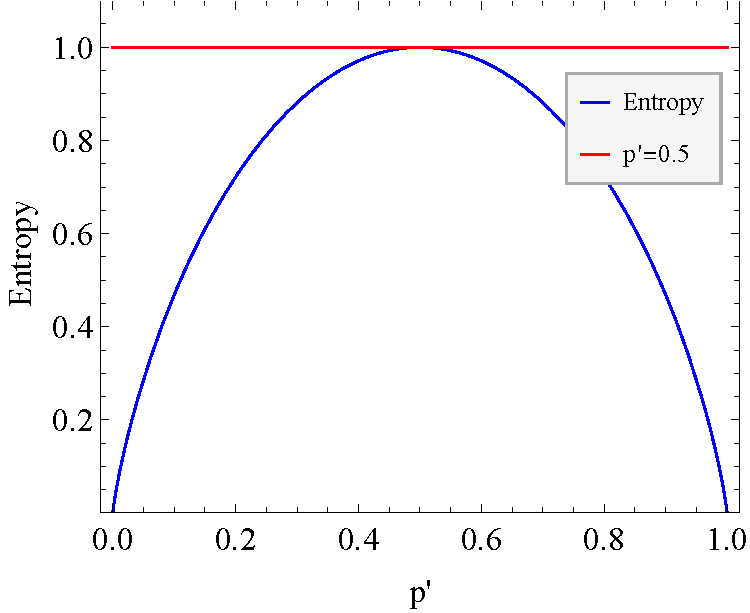
\includegraphics[width=0.8 \linewidth]{entropy}
\caption{Information entropy of a BF}
\label{fig:entropy}
\end{figure}
% We need to use the\textit{theory of information entropy} to deduce the formula of $k$, thus introduce its basic principle first.

% \textbf{Information Entropy}: In information theory, information entropy is used to measure the uncertainty of a random variable. In this paper, it refers to the \textit{Shannon entropy} \cite{shannon}, which measures the value of the information contained in a message.  Entropy is typically measured in bits, nats, or bans \cite{entropy}. For a variable with $s$ events with the probabilities of $p_1$, $p_2$, ..., $p_s$. The information entropy is:

% \begin{equation}
% p'=\sum_{i=1}^{s}p_i  log_2 \dfrac{1}{p_i}
% \end{equation}

% Here we give some conclusions about information entropy:

% %1) 变量的不确定性越大,熵也就越大
% 1) For a random variable, the larger the uncertainty is, the bigger the information entropy will be.

% 2) For any variable or message, there is a maximum value of information entropy.

% 3) When there are some characteristics or regulations in the message, its information entropy is not the maximum.

% Rather than get the exact formula of FP probability, given the value of $m$ and $n$, we deduce the exact formula of the optimal $k$ which Bose's and Christensen's formula cannot get.

% According to the theory of information entropy, when there are some characteristics/regulations in the array of Bloom Filter, the information entropy is not the maximum, and the array can be still compressed without any information loss. Based on this, we have Theorem I.

% \textbf{Theorem 1: } For a Bloom Filter, if its information entropy is not the maximum, then it is not optimal in size.

% \begin{proof}
% Given a set with $n$ elements, we build a BF with parameters of $m_1$ and $k$, its FP probability is $f_1$. We can compute its entropy. Assuming the entropy is not the maximum, according to the theory of entropy, the BF can be compressed into a smaller one BF2 ($m2 (m2<m1)$ , $k$, $f2$) without any information loss. The FP probability of BF2 is $f_2$, and $f_1=f_2$, because no information is lost during the compression.
% \end{proof}

% In other words, originally we have $m_1$, $k$, when $m_1$ bits are compressed to $m_2$ bits, $n$, $k$ and $f$ are not changed. That is to say, $m_1-m_2$ memory is wasted, thus the value of $k$ is not optimal for the BF with $m$ bits.

% It can be concluded that when there is no characteristic/regulation in the array, its information entropy is the maximum, and the value of $k$ is optimal given $m$ and $n$. Obviously, when the probability that every bit in the BF is 1 is 0.5, it has no characteristic/regulation, its information entropy reaches the maximum, and the value of $k$ is the optimal - $k^*$:
\begin{equation}
p'=\left(1-\frac{1}{m}\right)^{k^* n}=0.5
\label{equ:p=0.5}
\end{equation}
%$$
which is derived previously with the first independence assumption that is not disputed, we obtain:
\begin{equation}
\label{kform}
k^*=\dfrac{\ln 2}{n} \times \dfrac{1}{\ln m-\ln (m-1)} 
\end{equation}
This formula is very close to the formula of $k^*$ obtained by Bloom. As we have, as for small values of $x$, the approximation $\ln (1+x)\approx x$, and therefore $\ln m-\ln (m-1) \approx \frac{1}{m}$ yielding the same term as in Eq. \ref{eq:kopt}. 
%\textcolor{red}{In order to evaluate this approximation, we show in Figure~\ref{eva:err:m}, the approximation error, i.e., the difference, divided by $m$, between $1/(lnm-ln(m-1))$ and $m$ when $m$ becomes large. As can be seen, the difference between the two terms becomes around 0.5, which is in the order of a rounding error of the value of $k^*$.} This also means that using the Bloom formula Eq. \ref{eq:kopt} will result in at most a difference of 1 compared to our derivation.

%\begin{figure}
%\centering
%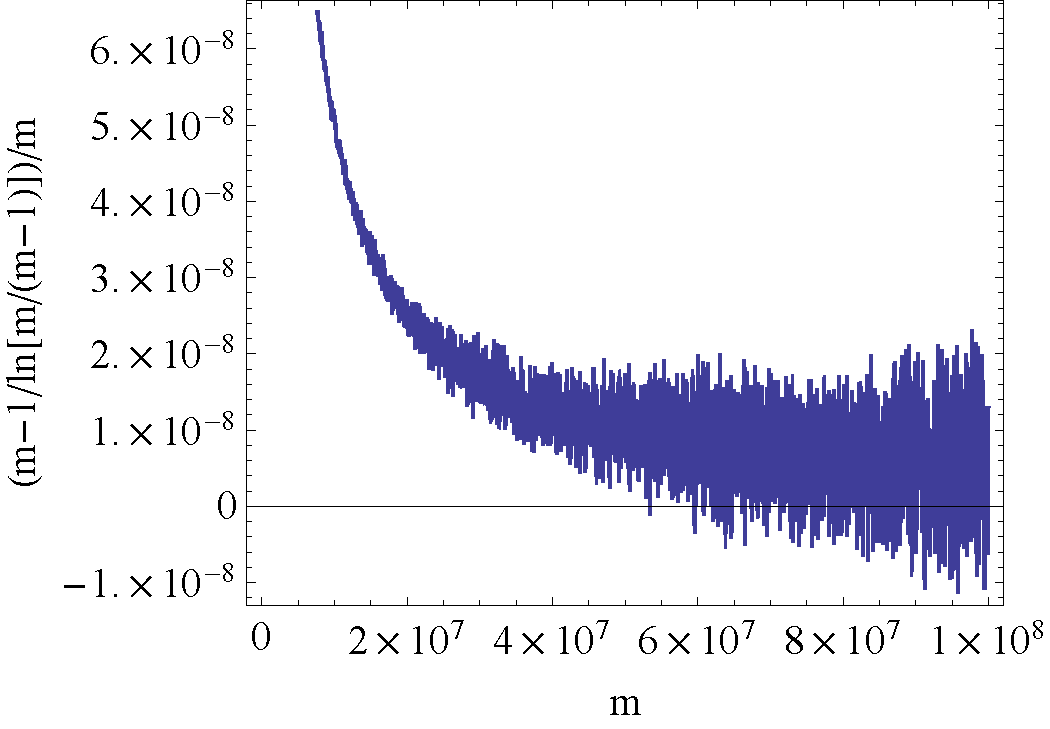
\includegraphics[width=0.8\linewidth]{error_m}
%\caption{The error of $k$ with the increase of $m$.}
%\label{eva:err:m}
%\end{figure}

%\section{Practicality of False Positive Calculation}

\section{Asymptotic Form of the False Positive Probability}
\label{sec:limitf}
We will derive a new and very simple approach to computing asymptotic form for the FP probability of Bloom Filters. The new derivation is based on \textit{partitioned Bloom Filters} (pBF) that are used frequently to carry out parallel query. Its principle is simple: the BF is divided into $k$ even partitions, and each hash function only acts on one of the partitions. %With this structure Using this method, there is a characteristic/regulation in the partitioned Bloom Filter: each partition of the Bloom Filter has at least one 1, thus its entropy is not the maximum.
The probability that one bit of the BF array remains 0 after inserting $n$ elements in the BF becomes
\begin{equation}
p'_{partition} = \left( 1-\dfrac{k}{m} \right)^n
\end{equation}
as now each hash maps into $\frac{m}{k}$ separate bits.

\textbf{Lemma:} For $m > 1 \;\;,   k >1 \;\; and \;\; n > 1$,
\begin{equation}
\label{theorem1}
\left( 1-\dfrac{k}{m} \right)  ^n <
\left( 1-\dfrac{1}{m} \right)  ^{kn}
\end{equation}
\begin{proof}
Let $g(k)=( 1-\frac{1}{m} )  ^k- ( 1-\frac{k}{m} )$. For $k>1$, $g(k)$ is a continuous and derivable function and its derivative is:
\begin{equation}
%g'(k)=k\left( 1- \dfrac{1}{m}\right) ^{k-1} +\dfrac{1}{m}
g'(k)=\left( 1- \dfrac{1}{m}\right)^k \ln\left(1-\dfrac{1}{m}\right)+\dfrac{1}{m}
\end{equation}
Since $m > 1$, $k > 1$, based on the derivative, we have:
\begin{equation}
\begin{aligned}
%g'(k)=k\left( 1- \dfrac{1}{m}\right) ^{k-1} +\dfrac{1}{m}
g'(k) &=\left( 1- \dfrac{1}{m}\right)^k \ln\left(1-\dfrac{1}{m}\right)+\dfrac{1}{m} \\
&> \left( 1- \dfrac{1}{m}\right)\ln\left(1-\dfrac{1}{m}\right)+\dfrac{1}{m}
\end{aligned}
\end{equation}
Let $f(m)=\left( 1- \dfrac{1}{m}\right)\ln\left(1-\dfrac{1}{m}\right)+\dfrac{1}{m}$, we can show $f'(m) = \dfrac{1}{m^2} \ln\left(1-\dfrac{1}{m}\right)< 0$, meaning that the function $f(m)$ is strictly decreasing. However, when $m$ goes to infinity, we have $\lim\limits_{m \to \infty}  f(m) =  0$. Therefore, we know that $f(m) \geq 0$, and $g'(k) > f(m) \geq 0$, meaning that the function $g(k)$ is strictly increasing.
%$f(m) \geq f(2)=\dfrac{1}{2} - \dfrac{1}{2}\ln\left(\dfrac{1}{2}\right)$. 
We have therefore 
\begin{equation}
0<\left( 1-\dfrac{k}{m} \right)   <
\left( 1-\dfrac{1}{m} \right)  ^k
\end{equation}
or 
\begin{equation}
\left( 1-\dfrac{k}{m} \right) ^n   <
\left( 1-\dfrac{1}{m} \right)  ^{kn}
\end{equation}
\end{proof}

%%%%%%%%%%%%%%%%%%%%%%%%%%%%%%%%%%%%%%%%%By Qiaobin%%%%%%%%%%%%%%%%%%%%%%%%%%%%%%%
%The above lemma shows that $p'_{partition} < p'_{true}$ or equivalently $1-p'_{partition} > 1-p'_{true}$. The probability that one bit of the array is set to 1 in a pBF of size $m$, and with $k$ hash functions is therefore larger than that of Bloom filter with same parameters, meaning that the pBF will in average have more bits set than an equivalent BF, and finally the FP probability of the pBF will be larger than the one of the equivalent BF.
According to the Information Theory, having characteristic means that the information entropy is not the maximum. From \textbf{Theorem II}, we know that the FP probability $f_{partition}$ is larger than the standard Bloom Filter  $f_{true}$, i.e., $f_{partition} > f_{true}$. In addition, Christensen’s bounds in Eq. \ref{fBound} state that the precise value of FP probability for a BF $f_{true}$ is larger than $f_{bloom}$, i.e., $f_{true} > f_{bloom}$.
%%%%%%%%%%%%%%%%%%%%%%%%%%%%%%%%%%%%%%%%%By Qiaobin%%%%%%%%%%%%%%%%%%%%%%%%%%%%%%%

%Having characteristic means that the information entropy is not the maximum, thus the FP probability $f_{partition}$ is larger than the standard Bloom Filter  $f_{true}$, thus we get
%However, Christensen’s bounds in Eq. \ref{fBound} state that the precise value of FP probability for a BF $f_{true}$ is larger than $f_{bloom}$, meaning that

Therefore, we have the following upper and lower bounds:
\begin{equation}
\label{bigbig}
f_{partition} > f_{true} > f_{bloom}
\end{equation}



For partitioned Bloom Filter, the probability that one bit of the array is still 0 is:

\begin{equation}
p'_{partition}=\left( 1-\dfrac{k}{m} \right)^n
\end{equation}

Different from standard Bloom Filter, for partitioned Bloom Filter, the event ``$E(h_1=1),E(h_2=1),E(h_3=1),...,E(h_{i-1}=1)$'' is independent with the event ``$E(h_{i-1}=1)$'', where $E(h_{i-1}=1)$ means the event that the position of $h_{i-1}(x)$ is 1, because each hash function is responsible for one partition, and has no effect with each other. Therefore, 

\begin{equation}
f_{partition}=(1-p'_{partition})^k=\left( 1- \left( 1-\dfrac{k}{m} \right)^n \right) ^k
\end{equation}

then the formula~\ref{bigbig} becomes

\begin{equation}
\left( 1- \left( 1-\dfrac{k}{m} \right)^n \right) ^k > f_{true} > \left( 1- \left( 1-\dfrac{1}{m} \right)^{nk} \right) ^k
\end{equation}

Then we use the famous limit formula:

\begin{equation}
\lim\limits_{x \to \infty} \left( 1-\dfrac{1}{x}\right) ^{-x} = e
\end{equation}

%and then get

%%%%%%%%%%%%%%%%%%%%%%%%%%%%%%%%%%%%%%%%%By Qiaobin%%%%%%%%%%%%%%%%%%%%%%%%%%%%%%%
%One can easily derive the FP probability for pBF as:
%\begin{equation}
%f_{partition}=(1-p'_{partition})^k=\left( 1- \left( 1-\dfrac{k}{m} \right)^n \right) ^k
%\end{equation}
%Different from standard Bloom Filter, the second independence assumption (the independence between the value of positions mapped by different hash functions) is valid as each hash accesses a bit in a different partition, therefore the above formula is precise resulting in the below upper and lower bounds for $f_{true}$: 

%\emph{Note that the above formula is the correct form of the pBF's FP probability, since all the $k$ hashings access different bits in different partitions, which guarantees that all the $k$ queried bits are independent and satisfies the ``multiple principle''.}
%Therefore, the formula~\ref{bigbig} becomes
%\begin{equation}
%\left( 1- \left( 1-\dfrac{k}{m} \right)^n \right) ^k > f_{true} > \left( 1- \left( 1-\dfrac{1}{m} \right)^{nk} \right) ^k
%\end{equation}
%%%%%%%%%%%%%%%%%%%%%%%%%%%%%%%%%%%%%%%%%By Qiaobin%%%%%%%%%%%%%%%%%%%%%%%%%%%%%%%

Asymptotically when $m$ becomes large, we already know that $f_{bloom}$ converges to the term in Eq. \ref{fBloom}. Nevertheless, the upper bound has also an asymptotic behaviour as :
\begin{equation}
\label{flim}
%\begin{aligned}
\lim\limits_{m \to \infty} \left(1-\left(1-\frac{1}{m}\right)^{nk}\right)^k = \left(1-e^{-nk/m}\right)^k 
%\end{aligned}
\end{equation}
that is the same term as the lower bound limit. Through \textbf{Sandwich Theorem} we get, similarly to Christensen and to Bose, that :
\begin{equation}
\label{flimtrue}
\lim\limits_{m \to \infty}  f_{true} =  \left(1-e^{-nk/m}\right)^k 
\end{equation}
This means that when $m$ is large, the Bloom's formula can be used with negligible error. However, we still need to evaluate what means \textit{$m$ being large}. We will do this by comparing the two bounds we have in hand: the one from Bose and the one we derived in this paper. 

\begin{figure}
\centering
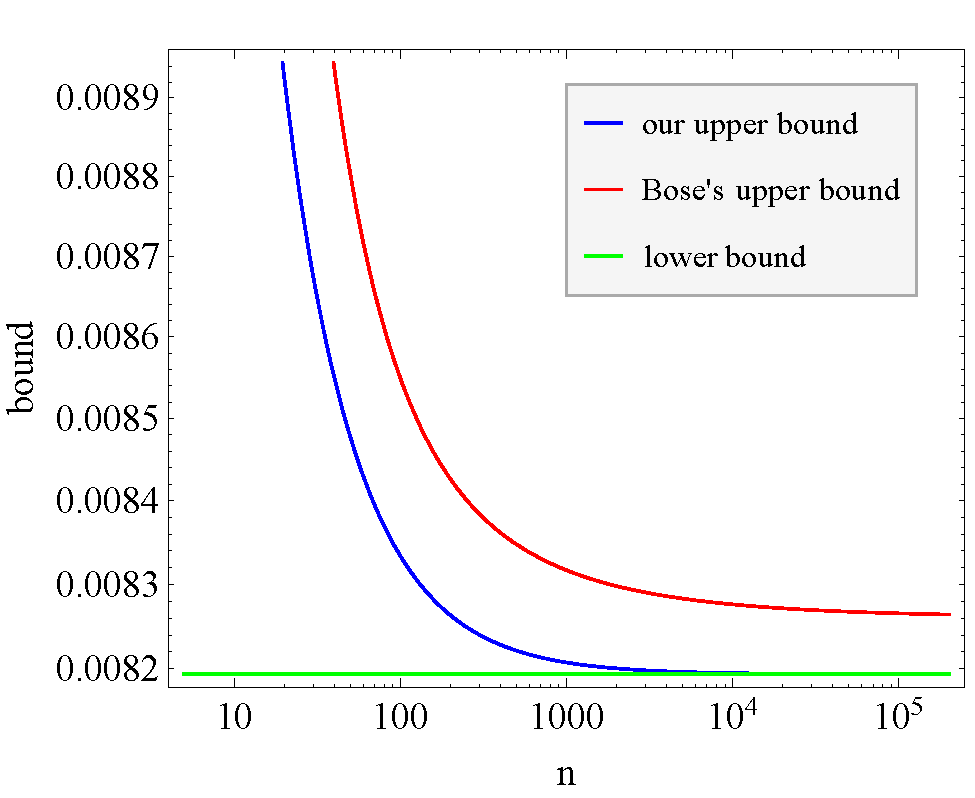
\includegraphics[width=0.8\linewidth]{LogLog_lowerUpper}
\caption{Upper and lower bound for $f_{true}$ for $k=7$ and $m=10n$.}
\label{fig:uplowbound}
\end{figure}

We show in Figure~\ref{fig:uplowbound} the two upper bounds along with the lower bound obtained for $k=7$  and $m=10n$ as a function of $n$, the number of elements inserted in the BF. As can be seen, the upper bound derived in this paper and the lower bound $p_{bloom}$ converge relatively fast for $n=9$, while the upper bound derived by Bose has a much slower convergence. We can see this better by looking at the behaviour of the bounds error ratio $\beta$, defined as $\beta=\frac{upper bound - lower bound}{lower bound}$, for the two bounds in Figure \ref{fig:ratio}
\begin{figure}
\centering
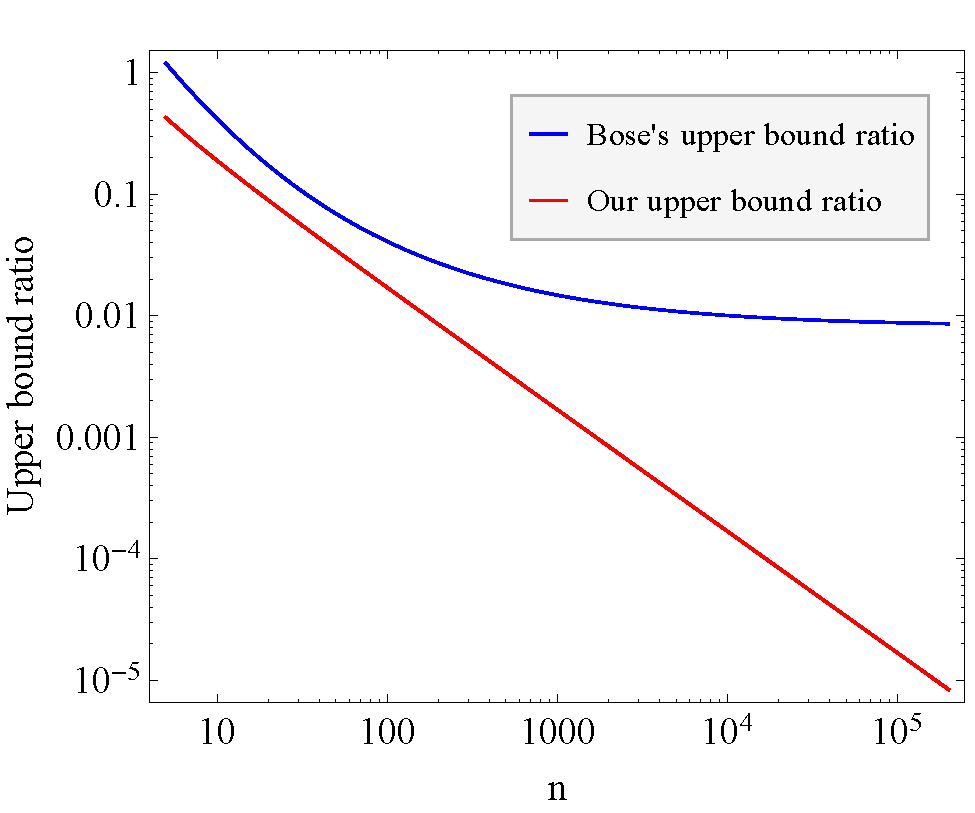
\includegraphics[width=0.8\linewidth]{LogLog_ratio}
\caption{Bounds error ratio for Bose's bound and the bound derived in this paper for $k=7$ and $m=10n$. }
\label{fig:ratio}
\end{figure}
As can be seen, the gap between the our derived upper bound and $f_{bloom}$ is decreasing polynomially at a constant speed, while Bose bound has a lower speed of convergence. In order to extend this observation, we show in Figure \ref{fig:ratiok} the evolution of the bounds error ratio for a BF with $m=10000$, $n=1000$ and varying $k$. 
\begin{figure}
\centering
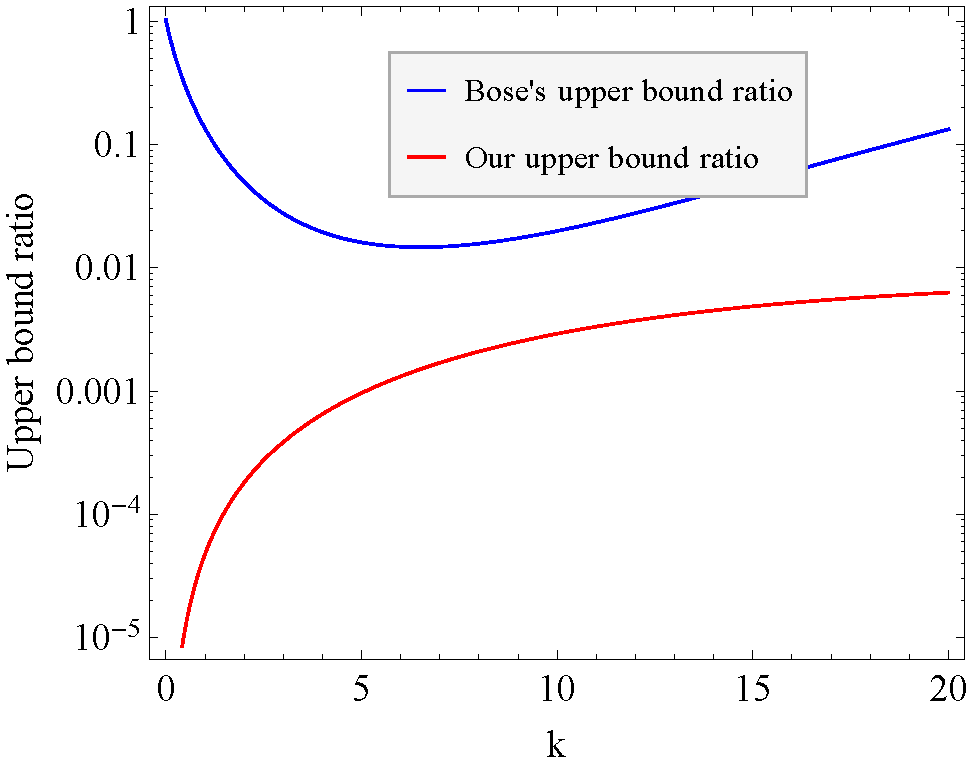
\includegraphics[width=0.8\linewidth]{ratioLog_k}
\caption{Bounds error ratio for Bose's bound and the bound derived in this paper for $m=10000$, $n=1000$ and varying $k$.}
\label{fig:ratiok}
\end{figure}
As expected, error involved with using $f_{bloom}$ increases with the number of hash functions $k$ increases. However, it can be seen that the convergence behaviour of the bounds derived in this paper is much better than the one obtained by Bose. 



 %\textbf{One Example.}
% \textbf{Example 1:}
%
% For example, $m=2, n=1, k=2$, the result using the Bloom's formula is 4.5/8.
% After hashing, there will be three cases: 10, 01, 11, thus the true false positive is 
%
% \begin{equation}
% \dfrac{1}{4}\times \dfrac{1}{4} +\dfrac{1}{4}\times \dfrac{1}{4} +1 \times \dfrac{2}{4}=\dfrac{5}{8}
% \end{equation} 
% In conclusion, the error of Bloom's formula is 1/16, when $m$ is 2.


% For example, $m=3, \, n=1,  \,  k=2$, there are three cases:
%
% Case I: two hashing map to the same position, the BF array will be one of the three: 100, 010, 001, each with the probability of 1/9. The FP probability of Case I is: 
%
% \begin{equation}
% (\dfrac{1}{3} \times \dfrac{1}{9} ) \times 3 = \dfrac{1}{9}
% \end{equation} 
% Case II: two hashings map to different positions, the BF array will be one of the three: 110, 101, 011, each with the probability of 2/9. First we compute the probability of no false positive:
%
% 1) Both the first and the second hashing positions are 0, the probability is 1/9.
%
% 2) The first hash position is 0, the second hash position is 1, the probability is 
% \begin{equation}
% \dfrac{1}{3} \times \dfrac{2}{3} = \dfrac{2}{9}
% \end{equation} 
%
% 3) The first hash position is 1, the second hash position is 0, the probability is also 2/9.
%
% Therefore, the probability of false positive of Case II is:
%
% \begin{equation}
% 1-\dfrac{1}{9}-\dfrac{2}{9}-\dfrac{2}{9}=\dfrac{4}{9}
% \end{equation}
%
% In sum, the probability of false positive of this example is:
%
%
% \begin{equation}
% \frac{1}{9}\times 3 \times \frac{1}{9}+ \frac{4}{9}\times 3\times \frac{2}{9}=\dfrac{27}{81}
% \end{equation}
%
% Note that the result using Bloom's formula is 25/81, and the error is 2/81.
%
%
%%套公式得出的结果是 25/81,误差是1/40.5
%%
%%\subsection{the results of suboptimal value}
%%For Standard Bloom Filter (SBF), the FP probability is given by:
%%
%%\begin{equation}
%%f=\left(1-\left(1-\dfrac{1}{m}\right)^{nk}\right)^k
%%\end{equation}
%%
%%When m is large, the formula reduces to
%%
%%\begin{equation}
%%\label{math:fpLargem}
%%f=\left(1-e^{-\dfrac{nk}{m}}
%%\right)^k
%%\end{equation} 